%section{The case for an IPv6 only LHCOPN}

The LHCOPN network implemented IPv6 quite early during its development. 
Since the start of IPv6 support in the EOS storage service, a large fraction of the data transfers carried by this network have changed Internet protocol, moving from IPv4 to IPv6. Since June 2019, LHCOPN carries more IPv6 packets than IPv4, as shown in figure~\ref{fig:lhcopne-traffic}.

\begin{figure}[h]
\centering
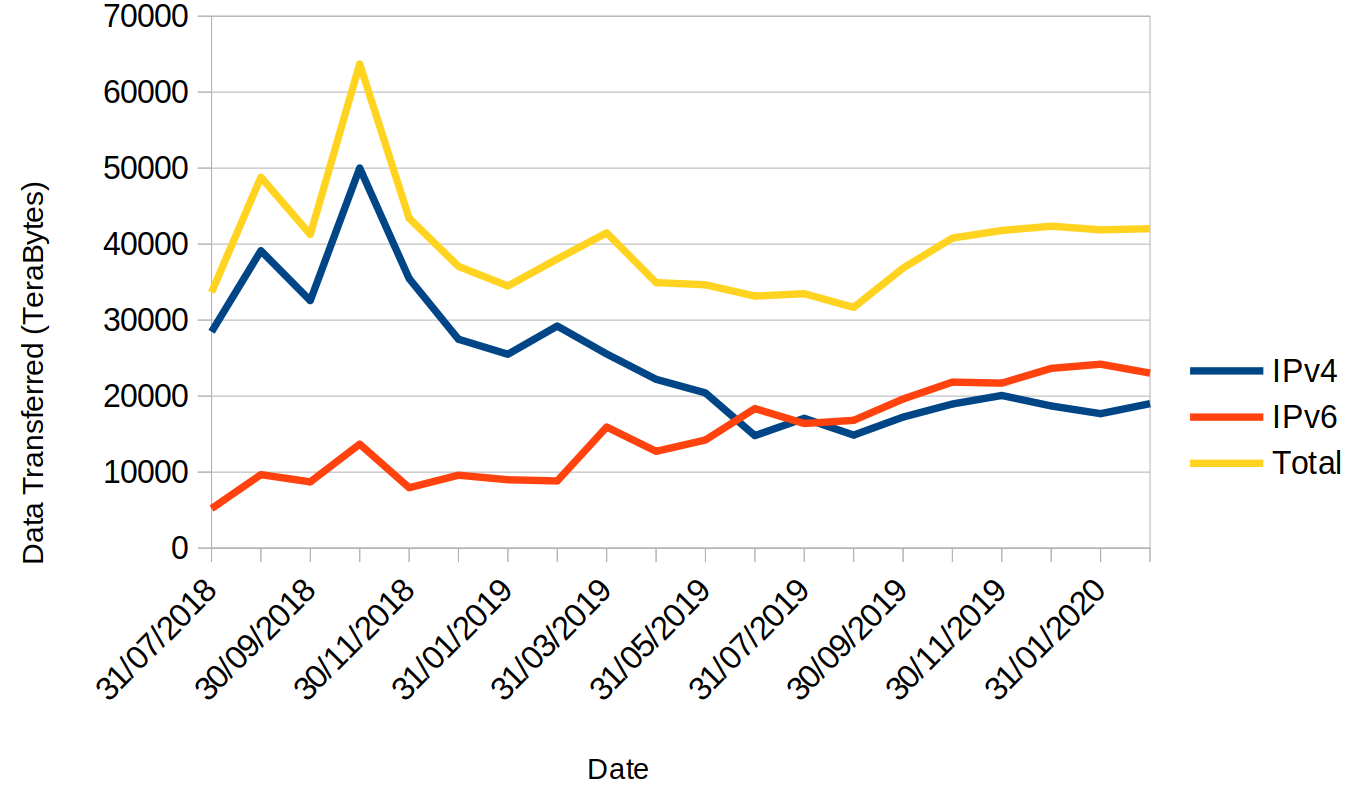
\includegraphics[width=8cm]{lhcopne-traffic.png}
\caption{LHCOPN and LHCONE IPv4-IPv6 traffic distribution as seen on the CERN routers\cite{RefLHCOPNEv4v6}  }
\label{fig:lhcopne-traffic}
\end{figure}

%\footnote{\href{https://twiki.cern.ch/twiki/bin/view/LHCOPN/LHCOPNEv4v6Traffic}{LHCOPN traffic comparison: https://twiki.cern.ch/twiki/bin/view/LHCOPN/LHCOPNEv4v6Traffic}}. 

It could be envisaged that in the near future, once all the Tier-1s will have implemented dual-stack storage services, the LHCOPN could be turned into an IPv6-only network. There are some advantages that an IPv6-only LHCOPN could bring:
\begin{itemize}
  \item Increased security: LHCOPN links connect directly into Tier-1 data-centres, often bypassing border firewalls. Removing one protocol would decrease the attack surface;
  \item Simpler operations: maintaining one transmission protocol would simplify the operation of the networks and the resolution of problems;
  \item More addresses: IPv6 provides a larger number of addresses which can be used to avoid NAT in all situation.
\end{itemize}

The HEPiX IPv6 Working Group will encourage the LHCOPN community to move to IPv6-only as soon as possible.




